\chapter{Diseño funcional y técnico}
\label{cap:diseno-funcional}

En este capítulo...

\section{Arquitectura de aplicaciones (alto nivel)}

La arquitectura definida para las aplicaciones destino y fuente que se
consideraron dentro del alcance del proyecto se muestran en la siguiente figura;
dentro de esta arquitectura de aplicaciones se consideró el proceso ETL que se
construyó.

\begin{figure}[htb]
  \begin{center}
    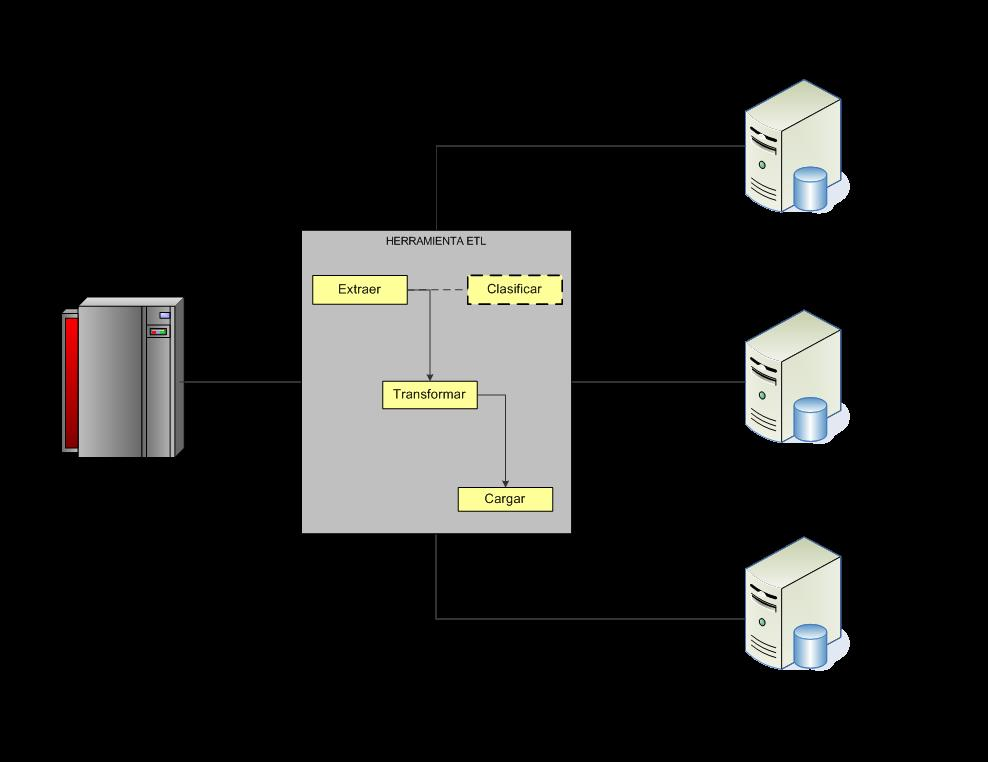
\includegraphics[width=12cm, height=3cm, scale=0.5]{Arquitectura.jpg}
        \caption{Arquitectura de aplicaciones.}
    \label{fig:arquitectura}
  \end{center}
\end{figure}

La arquitectura definida contenía al core bancario como sistema fuente de
información y enviaba la información a la herramienta ETL seleccionada para
realizar los procesos de extracción, transformación, clasificación y carga hacia
los sistemas destino y hacia cada uno de los tipos de datos que necesitaban los
equipos y bases de datos destino.

\section{Arquitectura de aplicaciones (arquitectura detallada)}

La arquitectura diseñada se encontraba dividida en cuatro capas y representan el
flujo de información entre cada una de dichas capas. La capa de interfaz de
usuario donde se realizaron todas las tareas de monitoreo, manejo de la
herramienta y visualización de datos en el sistema destino. La capa de
presentación únicamente contenía el servidor de correo que envía la información
a la capa de interfaz de usuario. Por su parte la capa de integración contenía
los procesos de la herramienta ETL; así como la base de datos \emph{stage} y la
base de datos de catálogos; esta capa también incluía a las aplicaciones que
enviaban información complementaria a los sistemas destino. Finalmente
contábamos con la capa de datos que contenía a los sistemas destino, el sistema
fuente y al servidor de control de usuarios a través del directorio activo. La
funcionalidad de cada capa así como el flujo de datos se describen a
continuación.

\subsection{Capa de datos}

La capa de datos contenía diferentes funcionalidades dependiendo del servidor de
datos del que estemos hablando. El core bancario tenía la funcionalidad de
enviar datos a la herramienta ETL a través del protocolo TCP\/IP. Por sus parte
el directorio activo al manejar información de los usuarios de la herramienta
tenía la funcionalidad de autenticar a cada usuario que accedía a la herramienta
otorgándole los permisos necesarios para ejecutar las tareas dentro de la
herramienta ETL, la comunicación entre la herramienta ETL y el directorio activo
se realizó mediante el protocolo LDAP.

Por su parte los sistemas destino deberían de tener la capacidad de recibir los
datos de parte de la herramienta ETL; así como de parte de los ETL's actuales de
la institución financiera y que complementaban la información del core bancario;
los sistemas destino reciben los datos mediante el protocolo TCP/IP
independientemente de la herramienta ETL que los envíe.

\subsection{Capa de integración}

La capa de integración tiene la funcionalidad de integrar los datos entre las
diferentes aplicaciones; la herramienta ETL contiene todos los servicios para la
extracción de datos del core bancario, transformarlos y cargarlos en los
diferentes sistemas destino de la capa de datos. La herramienta ETL tiene la
funcionalidad de enviar los datos a la base de datos \emph{stage}\footnote{Las
  bases de datos llamadas \emph{stage} son bases de datos temporales o de paso
  antes de llevar la información a su destino final.} así como a la base de
datos de catálogos. El proceso debía enviar vía FTP los archivos de texto a una
dirección específica dentro de un servidor para que el ETL del sistema
antilavado tome los archivos y complemente la información que será enviada vía
TCP/IP a la aplicación de usuario final. A su vez, el proceso ETL también envía
información a uno de los ETL's del sistema de reportes para que sea
complementada por parte del sistema de conciliación bancaria y sea enviada a la
base de datos final de reportes.

\subsection{Capa de presentación}

La capa de presentación de la institución financiera contenía solamente un
servidor de correo; la principal funcionalidad del servidor de correo era
proporcionar a los usuarios la información de los procesos; es decir, recibía
información del estado de los procesos ETL y a su vez enviaría la información
de este estado al usuario final.

\subsection{Capa de interfaz de usuario}

La funcionalidad de la capa de interfaz de usuario era administrar la
información que se recibe del servidor de correo así como de las diferentes
aplicaciones con las que contaba la institución financiera. Esta capa era capaz
de soportar un ambiente gráfico que permitía a los usuarios administrar,
construir y diseñar sus propios elementos.

\section{Tecnología conceptual}

A continuación definiremos el diseño conceptual de la arquitectura usada para el
proyecto, este diseño conceptual está dividido en cinco grandes áreas: Ambiente
de desarrollo, herramienta ETL, ambiente de operación, aplicaciones de la
institución financiera y la capa de infraestructura; de cada una de ellas
hablaremos durante este capitulo.

\begin{figure}[htb]
  \begin{center}
    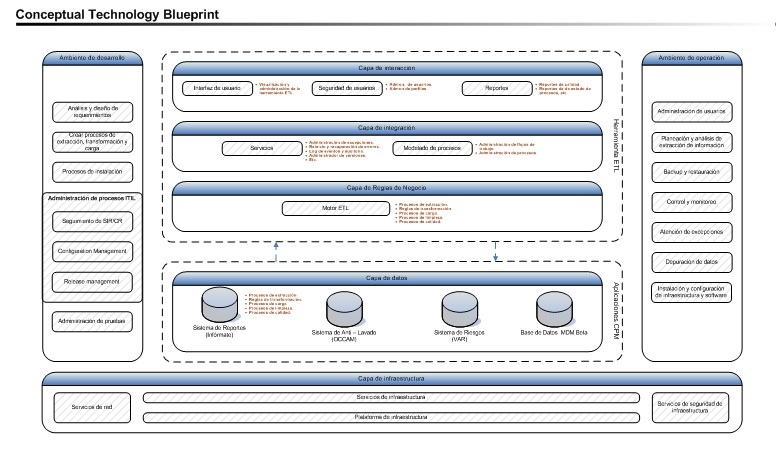
\includegraphics[width=12cm, height=4.5cm, scale=0.5]{Tecnologia_Conceptual.jpg}
        \caption{Tecnología conceptual.}
    \label{fig:conceptual}
  \end{center}
\end{figure}

\subsection{Ambiente de desarrollo}

Dentro del ambiente de desarrollo se encuentran definidas todas las actividades
que se requieren tener para la construcción de los procesos ETL, así como la
administración de los procesos y las pruebas. El ambiente de desarrollo tiene
los siguientes componentes:

\begin{itemize}

\item \textit{Análisis y diseño de requerimientos}: Dentro de la etapa de
  análisis y diseño de requerimientos encontramos la documentación de las
  fuentes y destinos de datos que serán procesadas mediante el ETL; el análisis
  de requerimientos abarca los requerimientos funcionales y técnicos que
  requiere la institución financiera para poder generar los datos en los
  sistemas destino.  Por su parte el diseño de los requerimientos incluyó el
  diseño funcional y técnico de todos los procesos a implementar dentro del ETL
  así como la definición de las reglas de programación y estándares que se
  tenían que seguir para un mejor desarrollo del proceso.

\item \textit{Creación de procesos de extracción, transformación y carga}: Una
  vez realizado el análisis y diseño de los procesos, el siguiente paso es
  construir los procesos ETL dentro de la herramienta seleccionada; para
  realizar este desarrollo se deberá de basar en el diseño funcional, en las
  reglas de transformación y en las reglas de negocio definidas dentro del
  propio diseño. El proceso de extracción para la primera iteración fue
  solamente del Core Bancario ICBS, mientras que las transformaciones y la carga
  se realizó de acuerdo al sistema al que se cargaron los datos.

\item \textit{Procesos de instalación}: Los procesos de instalación se refieren
  a los procesos a seguir para instalar el ETL dentro de los diferentes
  ambientes (desarrollo, pruebas y producción); este proceso también incluyó la
  instalación de la herramienta de ETL en la que se desarrollaron los procesos.
  Parte importante del proceso dentro del ambiente de desarrollo fue la
  administración de los procesos de ITIL, como parte de este proceso se tenía el
  seguimiento de reportes de incidencias (SIR) y controles de cambio (CR), la
  administración de configuraciones y la administración de versiones.

\item \textit{Reporte de incidencias y controles de cambio}: Se llevó a cabo un
  control de incidencias y control de cambios para todos los elementos
  desarrollados dentro del ETL.

\item \textit{Administración de configuraciones}. La administración de
  configuraciones fue parte importante dentro del ambiente de desarrollo por lo
  que fue necesario tener un registro de todas las configuraciones que se
  realizaron dentro de la herramienta.

\item \textit{Administración de versiones}. Toda herramienta ETL debe tener una
  administración de versiones para llevar el control de todos los cambios hechos
  en el desarrollo.

\item \textit{Administración de pruebas}: Como todo proyecto de implementación,
  fue necesario llevar una administración de las pruebas; las pruebas que se
  llevaron a cabo dentro de este proceso fueron: pruebas unitarias, pruebas de
  integración, pruebas de desempeño y pruebas de usuarios.

\end{itemize}

\section{Diseño de los programas ETL}

Como parte de la herramienta ETL se integraron tres áreas que tenían relación
con los requerimientos de negocio: la capa de interacción, la capa de
integración y la capa que contenía las reglas de negocio.

\begin{itemize}

\item Capa de interacción. Esta capa se refería a la interacción que tenían
  los usuarios con la herramienta ETL; así como la explotación de todos los
  elementos de la misma. Las principales funciones que se ejecutaron dentro de
  esta capa fueron la interfaz de usuario, la administración de protocolos de
  seguridad de usuarios y los reportes.

\item Capa de integración. En esta capa hicimos referencia a todos los
  servicios y modelado de procesos necesarios para el buen funcionamiento de
  nuestra herramienta ETL. Los principales procesos que se tomaron en cuenta
  fueron los siguientes:

  \begin{itemize}
  \item \textbf{Servicios}. Servicios necesarios para el manejo de errores,
    excepciones, versiones, así como servicios adicionales necesarios para los
    procesos de extracción, transformación y carga. Tales servicios se
    dividieron en: Administración de excepciones, reinicio y recuperación de
    errores, registros de eventos y auditoria y administración de versiones.
  \item \textbf{Modelado de procesos}. Fueron principalmente los procesos
    necesarios para la creación de los programas ETL.
  \end{itemize}

\item Reglas de negocio. Dentro de este proceso definimos las reglas para la
  transformación y carga correcta de los datos en la base de datos, así como la
  funcionalidad correcta que requería la entidad financiera. La principal
  herramienta que se tuvo en esta capa, fue el motor ETL y sus principales
  tareas fueron las siguientes:

  \begin{itemize}
  \item \textbf{Procesos de extracción.} Definición de todos los procesos
    utilizados para realizar la extracción de datos
  \item \textbf{Reglas de transformación.} Definición de todas las
    transformaciones utilizadas desde la extracción de datos hasta la carga de
    los mismos en la nueva estructura de base de datos.
  \item \textbf{Proceso de carga de datos.} Descripción de los procesos de carga
    de datos a cada uno de los sistemas destino.
  \item \textbf{Proceso de limpieza de datos.} Descripción de los procesos de
    limpieza de datos como: direcciones, teléfonos, nombres, RFCs y fechas.
  \item \textbf{Procesos de calidad.} Descripción de los procesos a seguir de
    acuerdo a los estándares de datos para tener una mejor calidad en la
    información.
  \end{itemize}

\end{itemize}

\section{Capa de datos}

La capa de datos estaba conformada por los diferentes sistemas desde donde se
extrajo la información así como los sistemas donde se almacenarían los
datos. Como sistema para extracción de datos solo se consideró un sistema,
mientras que la carga se realizó hacia tres diferentes sistemas de la
institución financiera. A continuación describo el tipo de información que se
procesaba en cada uno de los sistemas destino:

\begin{itemize}

\item Se tenía el sistema de detección de fraudes o posible mal manejo de una
  cuenta; esta detección se realizaba mediante el monitoreo de las cuentas que
  se enviaban a cada uno de los archivos generados por el procesador principal
  de transacciones bancarias.

\item El sistema de manejo de riesgos contenía la información de las cuentas
  con pagos vencidos o que presentaban algún grado de morosidad. Esta
  información también se obtenía del procesador principal de transacciones
  bancarias y sería procesada por la herramienta ETL que se implementó.

\item Finalmente, existía el sistema para el manejo de los reportes operativos
  que requería la organización. La principal tarea de este sistema era generar
  reportes regulatorios previamente definidos, así como extracción de
  información bajo demanda.
\end{itemize}

\cleardoublepage

%%% Local Variables:
%%% TeX-master: "Tesis"
%%% End:
